\apendice{Estudio experimental}

\section{Cuaderno de trabajo}

Este apartado detalla los métodos y técnicas probados a lo largo del desarrollo del proyecto, incluyendo tanto aquellos que arrojaron resultados positivos como los que no. Se documentaron meticulosamente los parámetros ajustados, resultados obtenidos, y las conclusiones derivadas. A continuación se enumeran los métodos y técnicas clave explorados:

\begin{itemize}
\item \textbf{Implementación de sensores AD8232 y su integración con Arduino}: Se realizaron pruebas de detección y filtrado de señales con el sensor AD8232, obteniendo buenos resultados en la amplificación y limpieza de las señales de ECG. Anteriormente, se experimentó con el sensor KY039, pero se descartó debido a su mayor sensibilidad al ruido y menor comodidad de uso.
\item \textbf{Pruebas de conexión Bluetooth con módulos HC-05}: Se realizaron ensayos para la transmisión de datos entre el hardware y la aplicación web. No obstante, se abandonó el uso del Bluetooth debido a problemas en la transmisión de valores float a la ventana de Tkinter.
\item \textbf{Desarrollo y optimización de la interfaz web}: Se probaron diversas versiones de la interfaz para mejorar la experiencia del usuario.
\item \textbf{Modelos de predicción de machine learning}: Se experimentó con varios algoritmos incluyendo Random Forest, ANN (Redes Neuronales Artificiales), Decision Tree, SVM (Máquinas de Soporte Vectorial) y KNN (K-Vecinos más Cercanos) para la clasificación de latidos cardíacos. Se seleccionó Random Forest por su precisión y adaptabilidad al proyecto.
\end{itemize}

Estos métodos se ajustaron y modificaron a lo largo del proyecto, buscando la optimización continua de los procedimientos y la mejora de los resultados finales.

\section{Detalle de resultados}

Este anexo presenta los resultados de la encuesta SUS (System Usability Scale), completada por una persona que no conocía de nada este proyecto y lo ha probado por primera vez el proyecto desarrollado. La encuesta tiene 10 preguntas, cada una con una escala de 1 a 5 como se puede observar en las figuras de abajo. Estos han sido los resultados de cada pregunta y el calculo de la puntuación SUS:

\begin{figure}[h]
\centering
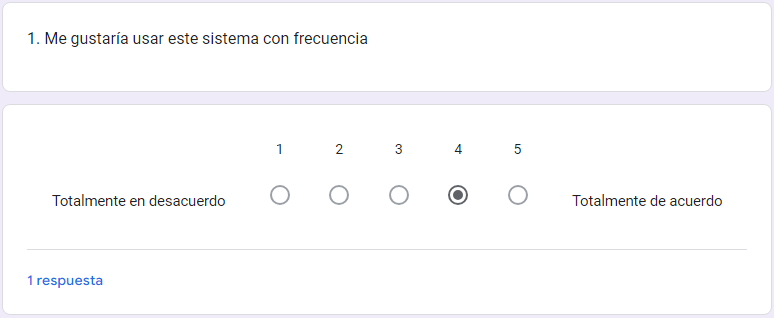
\includegraphics[width=1\textwidth]{img/Encuesta/1.png}
\caption{Encuesta SUS: Pregunta 1}
\label{fig:1}
\end{figure}

\begin{figure}[h]
\centering
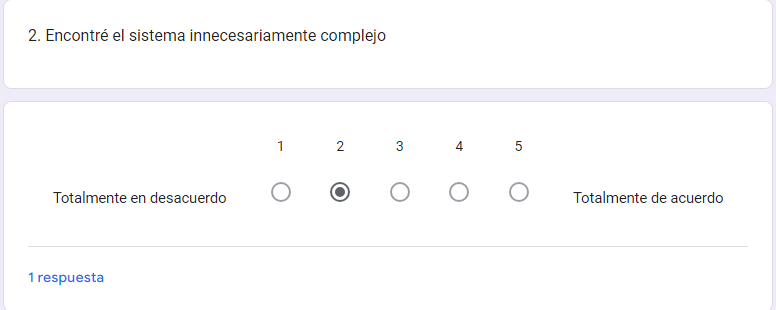
\includegraphics[width=1\textwidth]{img/Encuesta/2.png}
\caption{Encuesta SUS: Pregunta 2}
\label{fig:2}
\end{figure}

\begin{figure}[h]
\centering
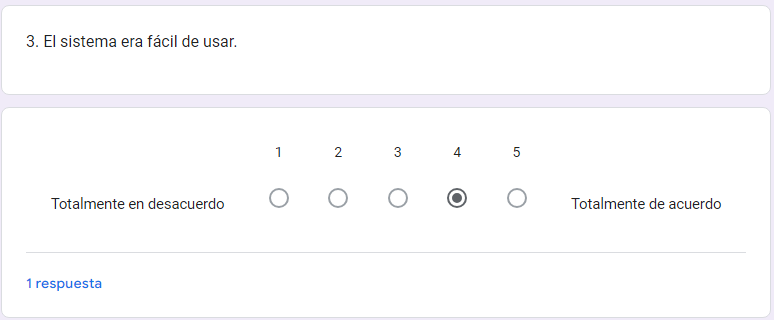
\includegraphics[width=1\textwidth]{img/Encuesta/3.png}
\caption{Encuesta SUS: Pregunta 3}
\label{fig:3}
\end{figure}

\begin{figure}[h]
\centering
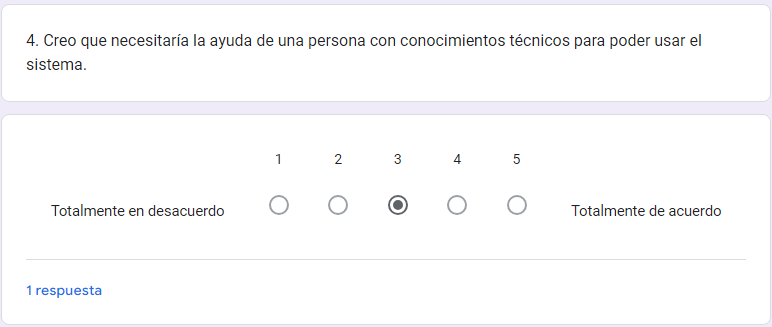
\includegraphics[width=1\textwidth]{img/Encuesta/4.png}
\caption{Encuesta SUS: Pregunta 4}
\label{fig:4}
\end{figure}

\begin{figure}[h]
\centering
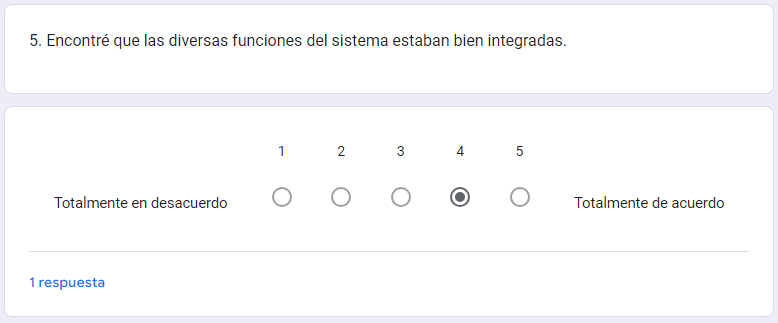
\includegraphics[width=1\textwidth]{img/Encuesta/5.png}
\caption{Encuesta SUS: Pregunta 5}
\label{fig:5}
\end{figure}

\begin{figure}[h]
\centering
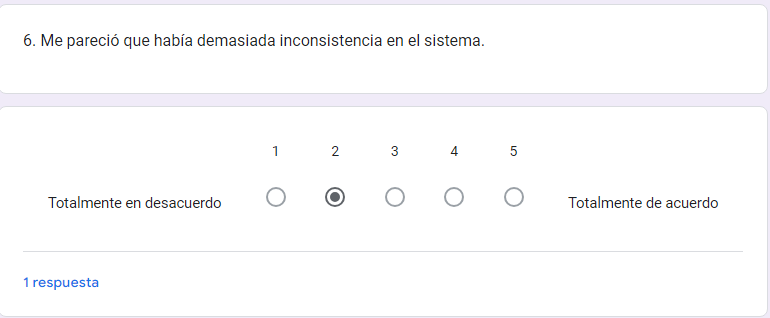
\includegraphics[width=1\textwidth]{img/Encuesta/6.png}
\caption{Encuesta SUS: Pregunta 6}
\label{fig:6}
\end{figure}

\begin{figure}[h]
\centering
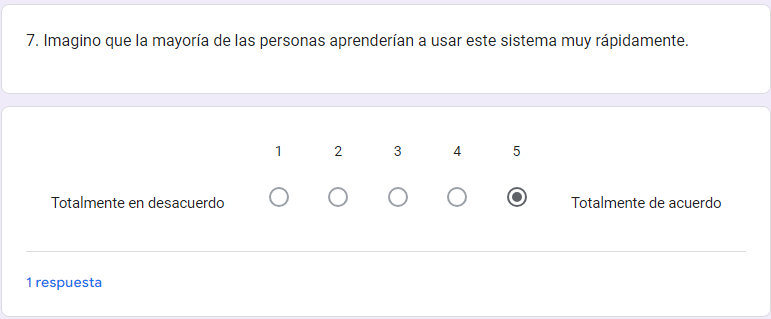
\includegraphics[width=1\textwidth]{img/Encuesta/7.png}
\caption{Encuesta SUS: Pregunta 7}
\label{fig:7}
\end{figure}

\begin{figure}[h]
\centering
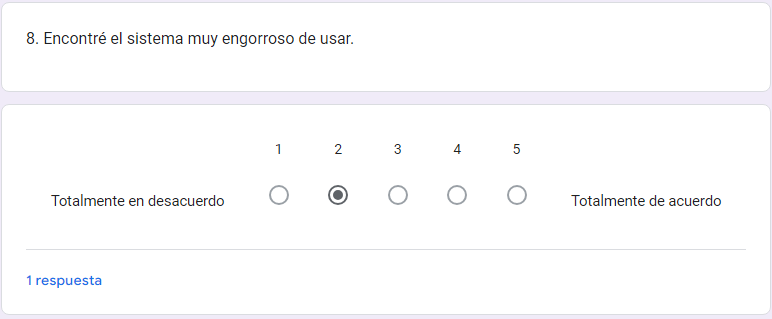
\includegraphics[width=1\textwidth]{img/Encuesta/8.png}
\caption{Encuesta SUS: Pregunta 8}
\label{fig:8}
\end{figure}

\begin{figure}[h]
\centering
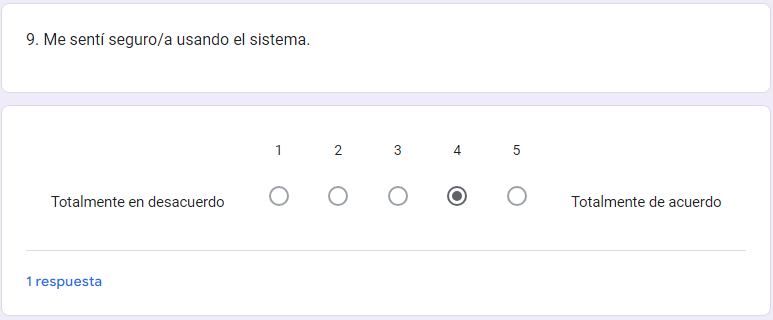
\includegraphics[width=1\textwidth]{img/Encuesta/9.png}
\caption{Encuesta SUS: Pregunta 9}
\label{fig:9}
\end{figure}

\begin{figure}[h]
\centering
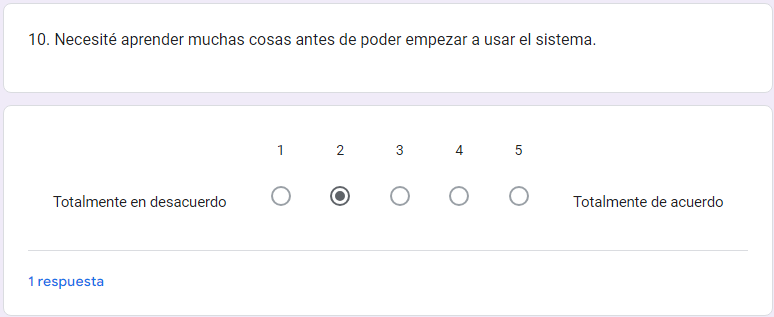
\includegraphics[width=1\textwidth]{img/Encuesta/10.png}
\caption{Encuesta SUS: Pregunta 10}
\label{fig:10}
\end{figure}

Para calcular la puntuación SUS hay que seguir los siguientes pasos \cite{SUS}:


\begin{enumerate}
\item Sumar las puntuaciones de cada pregunta  usando estas reglas:
\begin{itemize}
\item Para las preguntas 1, 3, 5, 7 y 9, la puntuación hay que restar 1, porque son preguntas que queremos que estén totalmente de acuerdo.
\item Para las preguntas 2, 4, 6, 8 y 10, la puntuación es 5 menos la posición en la escala. ya que son preguntar que lo ideal es que no estén de acuerdo.
\end{itemize}
\item La puntuación final se obtiene de multiplicar la suma total por 2.5.
\end{enumerate}

En este caso, los resultados son los siguientes:

\begin{itemize}
    \item Puntuaciones de las preguntas positivos (Preguntas 1, 3, 5, 7 y 9): 3, 3, 3, 4, 3
    \item Puntuaciones de las preguntas negativos (Preguntas 2, 4, 6, 8 y 10): 3, 3, 2, 3, 3
\end{itemize}

Suma total:
\[
(4+4+4+5+4) + (3+3+2+3+3) = 30
\]

Puntuación SUS:
\[
30 \times 2.5 = 75
\]

Este resultado de 75 sobre 100 indica que la usabilidad del sistema es bastante buena, ya que esta por encima de 68, que es el punto de referencia que consideraría que la web cumple bien los objetivos.
